\subsection{Decodificaci\'on Esteganogr\'afica (decode)}
	\subsubsection{Idea}
	
		Existe un m\'etodo de encriptaci\'on de mensajes llamado Esteganograf\'ia que consiste en utilizar im\'agenes para ofuscar o ocultar el mensaje haciendo casi imperceptibles cambios a las im\'agenes. En nuestro caso, sabemos exactamente como est\'an ocultos los mensajes y adem\'as sabemos el tama\~no del mensaje.
		
		Los caracteres del mensaje est\'an codificados en 4 bytes cada uno; extrayendo de cada byte 2 bits para armar el caracter de 8 bits. Tambi\'en hay que tener presente que hay otros 2 bits en cada uno de esos 4 bytes que indican si hay que cambiarle algo a los bits que forman el caracter.
		 
	\subsubsection{Implementaci\'on en C}

	El siguiente pseudocodigo resume la implementaci\'on en C:
	
	\begin{algorithmic}[1]
		\State unsigned char $caracter$ $\gets$ 0;
		\State int $cursor$ $\gets$ 0;
		\State int $pixelActual$ $\gets$ 0;
		\While{$size$-$cursor$ > 0}
			\State unsigned char $losCuatro$[4];
			\State cargar4Valores($losCuatro$,$cursor$,$src$);
			\For{int $i$ $\gets$ 0; $i$ < 4; $i$++} 
				\State $caracter$ $\gets$ $caracter$ $<<$ 2;
				\State unsigned char $code$ = obtenerCode($losCuatro$[3-$i$]);
				\State unsigned char $mod$ = obtenerMod($losCuatro$[3-$i$]);
				\State modificarCode($code$,$mod$);
				\State $caracter$ $\gets$ $caracter$ + $code$
			\EndFor
			\State guardarCaracter(caracter,cursor,dst);
			\State $pixelActual$ $\gets$ $pixelActual$ + 4
			\State $cursor$ $\gets$ $cursor$ + 1
		\EndWhile	
	\end{algorithmic}
	
	donde: 
	\begin{itemize}
		\item cargar4Valores($arreglo$,$pos$,$src$) levanta 4 valores de $src$ a partir de $pos$ y los guarda en $arreglo$.
		\item obtenerCode($val$) extrae los 2 bits menos significativos de $val$.
		\item obtenerMod($val$) extrae los segundos 2 bits menos significativos de $val$.
		\item modificarCode($c$, $m$) cambia el valor de $c$ seg\'un el valor de $m$.
		\item guardarCaracter($caracter$,$pos$,$dst$) guarda $caracter$ en $dst$ en la posici\'on $pos$.
	\end{itemize}


	\subsubsection{Implementaci\'on en ASM}
	
		La implementaci\'on en $ASM$ sigue la misma l\'ogica, pero trabaja de a m\'as p\'ixeles y por lo tanto procesa m\'as car\'acteres por iteraci\'on.
		
		\begin{figure}[H]
			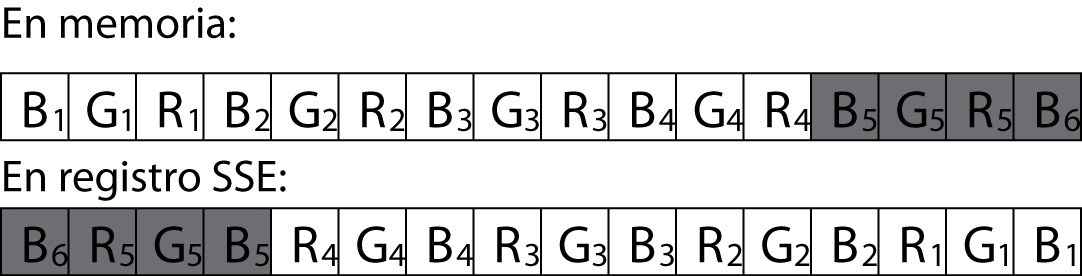
\includegraphics[scale=0.9]{imgs/fcolor_asm1.png} %Si, esta bien fcolor
			\caption{Al comienzo, tenemos en memoria los p\'ixeles con los caracteres codificados. Al cargar esos datos en un registro $SSE$ se observa que el orden de los elementos se invierte.} 
		\end{figure}
		
		\begin{figure}[H]
			
\includegraphics[scale=0.9]{imgs/decode_asm1.png} 
			\caption{Con estas m\'ascaras podemos extraer con $PAND$ los bits que nos interesan.} 
		\end{figure}
		
		\begin{figure}[H]
			
\includegraphics[scale=0.9]{imgs/decode_asm3.png} 
			\caption{Ya tenemos extra\'idos los $code$ y $mod$ de los 4 caracteres.}  
		\end{figure}
		
		
		Ahora, tenemos que hacer comparaciones para averiguar que tipo de $mod$ es para as\'i modificar el $code$ de forma acorde. Despu\'es de eso, acumulamos todos los $code$ ya modificados en un registro.
		
		\begin{figure}[H]
			
\includegraphics[scale=0.9]{imgs/decode_asm4.png} 
			\caption{Utilizando shifteos y sumas logramos acumular en determinadas posiciones los caracteres decodificados.}  
		\end{figure}
		
		\begin{figure}[H]
			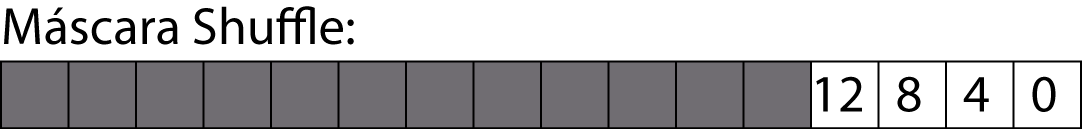
\includegraphics[scale=0.9]{imgs/decode_asm2.png} 
			\caption{Utilizando la siguiente m\'ascara para la instrucci\'on $PSHUFB$ podemos tener en la parte baja todos los caracteres juntos, para poder extraerlos m\'as f\'acilmente.}  
		\end{figure}
		
		Y luego, usando un registro de pr\'oposito general extraemos el conjunto de caracteres y los vamos insertando uno a uno en el mensajes $dst$, a medida que vamos disminuyendo $size$ del mensaje; si llega este valor a 0 en alg\'un momento durante la inserci\'on de los caracteres entonces ya termin\'o el mensaje y no tengo que seguir escribiendo.
		
		
	\subsubsection{Diferencias estructurales}
		Versión en C:

		-Procesa de a 4 bytes y por lo tanto obtiene un caracter por iteración.
		-Hay ciclos internos para cargar la información necesaria en arreglos.

		Versión en ASM:

		-Procesa de a 16 bytes y por lo tanto obtiene 4 caracteres por iteración.
		-No hay saltos condicionales más allá que los de escritura de caracteres y el del ciclo principal.
		-Acceder a los bits que componen a los números es más directo.


		A medida de que aumenta el tamaño de entrada se observa que la versión de ASM y su capacidad de procesar de a 4 caracteres impacta en el tiempo total de ejecución.

		Si la multiplicidad de filas y columnas no influye principalmente ya que se tiene como parámetro la longitud del mensaje a decodificar. Sin embargo, si no se cuenta con este dato entonces es preferible que las filas por las columnas de la imagen de entrada sean múltiplo de 16, ya que sino hay casos borde en donde al levantar de la imagen al registro se levanta basura que no pertenece a la imagen.

		//Analizar codigo generado por el compilador.
	\subsubsection{Optimizaciones de ASM}
	
	\paragraph{Software pipelining}
		La técnica de ''software pipelining'' es un método para optimizar ciclos en un código. La idea principal es emular en software la forma que tienen los procesadores modernos de hacer el ciclo de ''Fetch-Decode-Execute''. Los procesadores tienen un ''pipeline'' de instrucciones donde van concatenando instrucciones de procesador que no dependan una de la otra, y de esta manera aprovechar para ejecutar otras instrucciones mientras espera que instrucciones anteriores terminen.

		El compilador es aquel que se encarga de crear estas optimizaciones, aunque si el lenguaje es $assembler$ el programador es el responsable de realizar explícitamente esta técnica.

		Considere el siguiente programa en C:
		\begin{verbatim}
		for(i=0; i < cantIters; i++){
		    Inicio(i);
		    Nudo(i);
		    Desenlace(i);
		}
		\end{verbatim}

		donde Inicio(i), Nudo(i) y Desenlace(i) son instrucciones tales que dependen de la otra para procesar datos. Asimismo, esas instrucciones no dependen del parámetro $i$.

		El orden de ejecución de ese código es el siguiente:

		Inicio(0) $\Rightarrow$ Nudo(0) $\Rightarrow$ Desenlace(0) $\Rightarrow$ Inicio(1) $\Rightarrow$ Nudo(1) $\Rightarrow$ Desenlace(1) $\Rightarrow$ $\ldots$ 

		La técnica de ''software pipelining'' realiza una modificación al programa de la siguente manera:
		\begin{verbatim}
		for(i=0 ; i < (cantIters-3); i+=3){
		    Inicio(i);
		    Inicio(i+1);
		    Inicio(i+2);
		    Nudo(i);
		    Nudo(i+1);
		    Nudo(i+2);
		    Desenlace(i);
		    Desenlace(i+1);
		    Desenlace(i+2);
		}
		\end{verbatim}

		De manera que el nuevo orden de ejecución es:

		Inicio(0) $\Rightarrow$ Inicio(1) $\Rightarrow$ Inicio(2) $\Rightarrow$ 
		Nudo(0) $\Rightarrow$ Nudo(1) $\Rightarrow$ Nudo(2) $\Rightarrow$ 
		Desenlace(0) $\Rightarrow$ Desenlace(1) $\Rightarrow$ Desenlace(2) $\Rightarrow$ $\ldots$ 

		Cuando las instrucciones tienen tiempos de ejecución relativamente constante conseguimos una marcada mejoría en tiempo de ejecución total; una instrucción que para determinados parámetros tarda más en ejecutarse causa un cuello de botella y hace que aumente el tiempo de ejecución total.

		Una desventaja de este método es un alto uso de registros del procesador y por esta razón es que la aplicación de ''software pipelining'' al filtro $decode$ sólo puede ejecutar de a 2 conjuntos de instrucciones independientes a la vez.

		Hay momentos en que una parte del código carga una máscara de memoria para luego usarla para procesar los datos. Como estamos ejecutando dos conjuntos de instrucciones a la vez, fue beneficioso que el primer conjunto lo tome de memoria hacia un registro y luego copiar de dicho registro la máscara a otro registro para que el segundo conjunto de instrucciones no tenga que levantarlas de memoria nuevamente.

		Optimizaciones que se podrían realizar para reducir el ''overhead'' de los accesos a memoria es cargar de antemano las máscaras a registros determinados y no cambiarlos en ningún momento de la ejecución; sin embargo esto me limita la cantidad de registros disponibles y se necesitaría copiar datos de un registro a otro para poder resguardar la información de los registros.
		
	\subsubsection{An\'alisis temporal}